\documentclass[aspectratio=169]{beamer}

% Theme
\usetheme{default}
\usecolortheme{beaver}

% Packages
\usepackage{amsmath,amssymb,amsthm}
\usepackage{mathtools}
\usepackage{bm}
\usepackage{tikz}
\usetikzlibrary{arrows.meta,positioning,calc,patterns}

% Custom commands
\newcommand{\R}{\mathbb{R}}
\newcommand{\Pp}{\mathcal{P}}
\newcommand{\Mm}{\mathcal{M}}
\newcommand{\Ld}{\mathcal{L}^d}
\newcommand{\Cb}{C_b}

% Title
\title{Primal and Dual Problems}
\subtitle{Optimal Transport Theory}
\author{}
\date{}

\begin{document}

%==============================================================================
\begin{frame}
\titlepage
\end{frame}

%==============================================================================
\begin{frame}{Outline}
\tableofcontents[hideallsubsections]
\end{frame}

%==============================================================================
\section{Notation}
%==============================================================================

\begin{frame}{Notation: Spaces and Measures}
\textbf{Measure Spaces:}
\begin{itemize}
    \item $\Pp(X)$: probability measures on $X$
    \item $\Mm(X)$: finite signed measures on $X$
    \item $\Mm_+(X)$: positive finite measures on $X$
    \item $\Mm^d(X)$: vector measures (valued in $\R^d$) on $X$
\end{itemize}

\vspace{0.3cm}
\textbf{Special Measures:}
\[
\underbrace{\delta_a}_{\text{Dirac mass at } a}: \quad \delta_a(A) = \begin{cases} 1 & \text{if } a \in A \\ 0 & \text{if } a \notin A \end{cases}
\]

\vspace{0.2cm}
\begin{center}
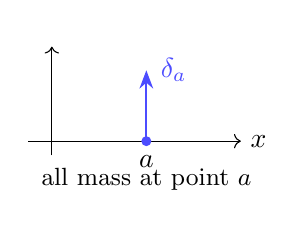
\begin{tikzpicture}[scale=0.6]
    \draw[->] (-0.5,0) -- (4,0) node[right] {$x$};
    \draw[->] (0,-0.3) -- (0,2) node[above] {};
    \fill[blue!70] (2,0) circle (3pt);
    \node[below] at (2,-0.1) {$a$};
    \draw[-{Stealth},blue!70,thick] (2,0) -- (2,1.5);
    \node[right,blue!70] at (2.1,1.5) {$\delta_a$};
    \node at (2,-0.8) {\small all mass at point $a$};
\end{tikzpicture}
\end{center}
\end{frame}

%==============================================================================
\begin{frame}{Notation: Indicator and Lebesgue Measure}
\textbf{Indicator Function:}
\[
\mathbb{1}_A(x) = \begin{cases} 1 & \text{if } x \in A \\ 0 & \text{if } x \notin A \end{cases}
\]

\vspace{0.3cm}
\textbf{Lebesgue Measure:}
\[
|A| = \Ld(A) = \int_A dx \quad \text{(volume of set } A \subset \R^d\text{)}
\]

\vspace{0.3cm}
\textbf{Density:} $f \cdot \mu$ denotes measure with density $f$ w.r.t. $\mu$:
\[
(f \cdot \mu)(A) = \int_A f \, d\mu
\]

\vspace{0.3cm}
\textbf{Restriction:} $\mu \llcorner A$ is $\mu$ restricted to set $A$ (i.e., $\mathbb{1}_A \cdot \mu$)
\end{frame}

%==============================================================================
\begin{frame}{Notation: Differential Operators}
\textbf{Gradient and Divergence:}
\[
\nabla u = \left( \frac{\partial u}{\partial x_1}, \ldots, \frac{\partial u}{\partial x_d} \right), \qquad \nabla \cdot \mathbf{v} = \sum_{i=1}^d \frac{\partial v_i}{\partial x_i}
\]

\vspace{0.3cm}
\textbf{Laplacian:}
\[
\Delta u := \nabla \cdot (\nabla u) = \sum_{i=1}^d \frac{\partial^2 u}{\partial x_i^2}
\]

\vspace{0.3cm}
\textbf{Hessian:} $D^2 u$ is the matrix of second derivatives:
\[
(D^2 u)_{ij} = \frac{\partial^2 u}{\partial x_i \partial x_j}
\]

\vspace{0.2cm}
\begin{center}
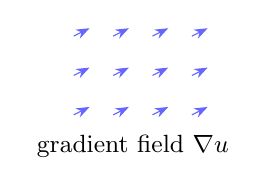
\begin{tikzpicture}[scale=0.5]
    \foreach \x in {0,1,2,3} {
        \foreach \y in {0,1,2} {
            \draw[-{Stealth},blue!60] (\x,\y) -- (\x+0.4,\y+0.2);
        }
    }
    \node at (1.5,-0.8) {\small gradient field $\nabla u$};
\end{tikzpicture}
\end{center}
\end{frame}

%==============================================================================
\begin{frame}{Notation: Transport}
\textbf{Push-forward (Image Measure):}
\[
T_\# \mu : \quad (T_\# \mu)(A) := \mu(T^{-1}(A))
\]

\vspace{0.2cm}
\textbf{Transport Plans:}
\[
\Pi(\mu, \nu) = \left\{ \gamma \in \Pp(X \times Y) : (\pi_x)_\# \gamma = \mu, \; (\pi_y)_\# \gamma = \nu \right\}
\]

\vspace{0.2cm}
\textbf{Product Measure:}
\[
(\mu \otimes \nu)(A \times B) = \mu(A) \cdot \nu(B)
\]

\vspace{0.2cm}
\textbf{Costs:}
\begin{itemize}
    \item $M(T)$: Monge cost of map $T$
    \item $K(\gamma)$: Kantorovich cost of plan $\gamma$
\end{itemize}

\vspace{0.2cm}
\textbf{Wasserstein:} $W_p(\mu,\nu)$ distance, $\mathcal{W}_p$ space
\end{frame}

%==============================================================================
\section{The Monge Problem}
%==============================================================================

\begin{frame}{The Monge Problem (1781)}
Given $\mu \in \Pp(X)$, $\nu \in \Pp(Y)$, and cost $c: X \times Y \to [0, +\infty]$:

\vspace{0.3cm}
\[
\textbf{(MP)} \quad \inf \left\{ M(T) := \int_X \underbrace{c(x, T(x))}_{\text{cost to move } x \to T(x)} \, d\mu(x) \;:\; \underbrace{T_\# \mu = \nu}_{\text{mass balance}} \right\}
\]

\vspace{0.4cm}
\begin{center}
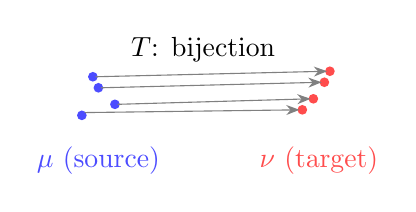
\begin{tikzpicture}[scale=0.7]
    % Source
    \foreach \x/\y in {0/0, 0.3/0.5, 0.6/0.2, 0.2/0.7} {
        \fill[blue!70] (\x,\y) circle (2.5pt);
    }
    \node[below,blue!70] at (0.3,-0.4) {$\mu$ (source)};

    % Target
    \foreach \x/\y in {4/0.1, 4.4/0.6, 4.2/0.3, 4.5/0.8} {
        \fill[red!70] (\x,\y) circle (2.5pt);
    }
    \node[below,red!70] at (4.3,-0.4) {$\nu$ (target)};

    % Arrows (one-to-one)
    \draw[-{Stealth},gray] (0.05,0.05) -- (3.95,0.1);
    \draw[-{Stealth},gray] (0.35,0.5) -- (4.35,0.6);
    \draw[-{Stealth},gray] (0.65,0.2) -- (4.15,0.3);
    \draw[-{Stealth},gray] (0.25,0.7) -- (4.45,0.8);

    \node at (2.2,1.2) {$T$: bijection};
\end{tikzpicture}
\end{center}
\end{frame}

%==============================================================================
\begin{frame}{Push-forward Measure}
\textbf{Definition:} For map $T: X \to Y$ and measure $\mu$ on $X$:
\[
(T_\# \mu)(A) := \mu\bigl(\underbrace{T^{-1}(A)}_{\text{preimage of } A}\bigr) \quad \text{for every measurable } A \subset Y
\]

\vspace{0.3cm}
\textbf{Integral form:} For any measurable $\phi: Y \to \R$:
\[
\int_Y \phi(y) \, d(T_\# \mu)(y) = \int_X \underbrace{\phi(T(x))}_{\text{composition}} \, d\mu(x)
\]

\vspace{0.3cm}
\begin{center}
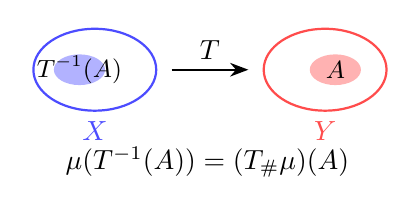
\begin{tikzpicture}[scale=0.65]
    % X space
    \draw[blue!70,thick] (0,0) ellipse (1.2 and 0.8);
    \node[blue!70] at (0,-1.2) {$X$};
    \fill[blue!30] (-0.3,0) ellipse (0.5 and 0.3);
    \node[font=\small] at (-0.3,0) {$T^{-1}(A)$};

    % Arrow
    \draw[-{Stealth},thick] (1.5,0) -- node[above] {$T$} (3,0);

    % Y space
    \draw[red!70,thick] (4.5,0) ellipse (1.2 and 0.8);
    \node[red!70] at (4.5,-1.2) {$Y$};
    \fill[red!30] (4.7,0) ellipse (0.5 and 0.3);
    \node[font=\small] at (4.7,0) {$A$};

    % Measure annotation
    \node at (2.2,-1.8) {$\mu(T^{-1}(A)) = (T_\# \mu)(A)$};
\end{tikzpicture}
\end{center}
\end{frame}

%==============================================================================
\begin{frame}{Difficulty: Mass Cannot Split}
\textbf{Problem:} A transport \emph{map} $T$ sends each point to exactly one destination.

\vspace{0.3cm}
\textbf{Example:} $\mu = \delta_0$, $\nu = \frac{1}{2}\delta_a + \frac{1}{2}\delta_b$

\vspace{0.3cm}
\begin{center}
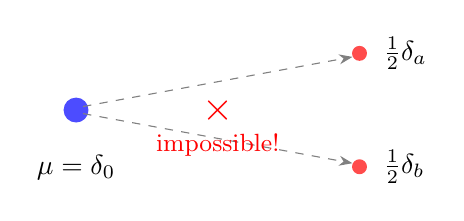
\begin{tikzpicture}[scale=0.9]
    % Source
    \fill[blue!70] (0,0) circle (5pt);
    \node[below] at (0,-0.5) {$\mu = \delta_0$};

    % Targets
    \fill[red!70] (4,0.8) circle (3pt);
    \node[right] at (4.2,0.8) {$\frac{1}{2}\delta_a$};
    \fill[red!70] (4,-0.8) circle (3pt);
    \node[right] at (4.2,-0.8) {$\frac{1}{2}\delta_b$};

    % Impossible arrows
    \draw[-{Stealth},gray,dashed] (0.1,0.05) -- (3.9,0.75);
    \draw[-{Stealth},gray,dashed] (0.1,-0.05) -- (3.9,-0.75);

    % X mark
    \node[red,font=\Large] at (2,0) {\textbf{$\times$}};
    \node[red] at (2,-0.5) {\small impossible!};
\end{tikzpicture}
\end{center}

\vspace{0.3cm}
$\Rightarrow$ \textbf{No transport map exists!} The constraint $T_\# \mu = \nu$ cannot be satisfied.

\vspace{0.2cm}
\textbf{Other issues:}
\begin{itemize}
    \item Constraint $T_\# \mu = \nu$ is \textbf{nonlinear}
    \item Not closed under weak convergence
\end{itemize}
\end{frame}

%==============================================================================
\section{Kantorovich Relaxation}
%==============================================================================

\begin{frame}{Kantorovich's Idea (1942)}
\textbf{Key insight:} Replace transport \emph{maps} with transport \emph{plans}.

\vspace{0.3cm}
A \textbf{transport plan} $\gamma$ on $X \times Y$ specifies: for each pair $(x,y)$, how much mass moves from $x$ to $y$.

\vspace{0.3cm}
\[
\gamma(A \times B) = \text{``mass moving from } A \text{ to } B\text{''}
\]

\vspace{0.3cm}
\textbf{Marginal constraints:}
\[
\underbrace{(\pi_x)_\# \gamma = \mu}_{\text{total mass leaving } x} \quad \text{and} \quad \underbrace{(\pi_y)_\# \gamma = \nu}_{\text{total mass arriving at } y}
\]

where $\pi_x(x,y) = x$ and $\pi_y(x,y) = y$ are projections.

\vspace{0.3cm}
\textbf{Advantage:} Mass can \textbf{split}! From one $x$, mass can go to multiple $y$'s.
\end{frame}

%==============================================================================
\begin{frame}{Kantorovich Problem (KP)}
\[
\textbf{(KP)} \quad \inf \left\{ K(\gamma) := \int_{X \times Y} c(x,y) \, d\gamma(x,y) \;:\; \gamma \in \Pi(\mu, \nu) \right\}
\]

\vspace{0.3cm}
where the set of \textbf{transport plans} is:
\[
\Pi(\mu, \nu) = \left\{ \gamma \in \Pp(X \times Y) : \underbrace{(\pi_x)_\# \gamma = \mu}_{\text{1st marginal}}, \; \underbrace{(\pi_y)_\# \gamma = \nu}_{\text{2nd marginal}} \right\}
\]

\vspace{0.4cm}
\textbf{Key advantages over (MP):}
\begin{itemize}
    \item \textbf{Linear} objective + \textbf{linear} constraints $\Rightarrow$ Linear Programming
    \item $\Pi(\mu, \nu) \neq \emptyset$ always (e.g., $\mu \otimes \nu \in \Pi(\mu, \nu)$)
    \item Existence guaranteed by weak-* compactness
    \item Mass splitting allowed!
\end{itemize}
\end{frame}

%==============================================================================
\begin{frame}{Transport Plan Visualization}
\begin{columns}
\begin{column}{0.5\textwidth}
\textbf{Monge map:}\\
$x \mapsto T(x)$ (one destination per $x$)

\vspace{0.5cm}
\textbf{Kantorovich plan:}\\
$\gamma(x,y)$ = mass from $x$ to $y$\\
(can split!)

\vspace{0.5cm}
\textbf{Connection:}\\
If $T$ is a map with $T_\# \mu = \nu$, then
\[
\gamma_T := (\text{id}, T)_\# \mu
\]
is a valid transport plan.
\end{column}
\begin{column}{0.5\textwidth}
\begin{center}
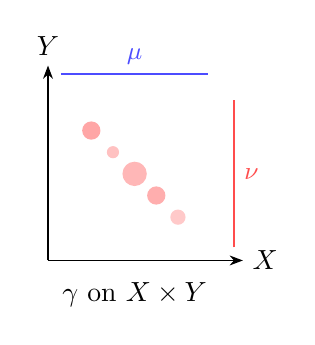
\begin{tikzpicture}[scale=0.55]
    \draw[-{Stealth}] (0,0) -- (4.5,0) node[right] {$X$};
    \draw[-{Stealth}] (0,0) -- (0,4.5) node[above] {$Y$};

    % Transport plan blobs
    \fill[red!50,opacity=0.7] (1,3) circle (6pt);
    \fill[red!40,opacity=0.7] (2,2) circle (8pt);
    \fill[red!30,opacity=0.7] (3,1) circle (5pt);
    \fill[red!35,opacity=0.7] (1.5,2.5) circle (4pt);
    \fill[red!45,opacity=0.7] (2.5,1.5) circle (6pt);

    \node at (2,-0.8) {$\gamma$ on $X \times Y$};

    % Marginal arrows
    \draw[blue!70,thick] (0.3,4.3) -- (3.7,4.3);
    \node[blue!70,font=\small] at (2,4.7) {$\mu$};

    \draw[red!70,thick] (4.3,0.3) -- (4.3,3.7);
    \node[red!70,font=\small] at (4.7,2) {$\nu$};
\end{tikzpicture}
\end{center}
\end{column}
\end{columns}
\end{frame}

%==============================================================================
\begin{frame}{Transport Plan from a Map}
If $T: X \to Y$ is a transport map (i.e., $T_\# \mu = \nu$), define:
\[
\gamma_T := (\text{id}, T)_\# \mu
\]

This means: $\gamma_T$ is concentrated on the \textbf{graph} of $T$.
\[
\gamma_T(A \times B) = \mu\bigl(\{x \in A : T(x) \in B\}\bigr)
\]

\vspace{0.3cm}
\textbf{Key property:}
\[
\int_{X \times Y} c(x,y) \, d\gamma_T = \int_X c(x, T(x)) \, d\mu(x) = M(T)
\]

\vspace{0.2cm}
\begin{center}
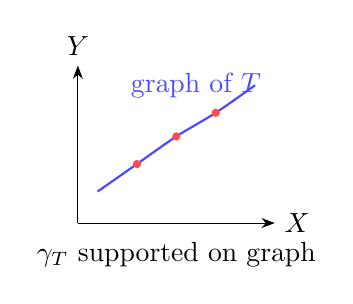
\begin{tikzpicture}[scale=0.5]
    \draw[-{Stealth}] (0,0) -- (5,0) node[right] {$X$};
    \draw[-{Stealth}] (0,0) -- (0,4) node[above] {$Y$};

    % Graph of T
    \draw[blue!70,thick] plot[smooth] coordinates {(0.5,0.8) (1.5,1.5) (2.5,2.2) (3.5,2.8) (4.5,3.5)};
    \node[blue!70] at (3,3.5) {graph of $T$};

    % Points on graph
    \fill[red!70] (1.5,1.5) circle (3pt);
    \fill[red!70] (2.5,2.2) circle (3pt);
    \fill[red!70] (3.5,2.8) circle (3pt);

    \node at (2.5,-0.8) {$\gamma_T$ supported on graph};
\end{tikzpicture}
\end{center}
\end{frame}

%==============================================================================
\begin{frame}{Exercise 1: Discrete Transport Plans}
\textbf{Problem:} Let $X = Y = \{1, 2\}$ with
\[
\mu = \frac{1}{2}\delta_1 + \frac{1}{2}\delta_2, \qquad \nu = \frac{1}{2}\delta_1 + \frac{1}{2}\delta_2
\]

A transport plan $\gamma \in \Pi(\mu, \nu)$ can be represented as a $2 \times 2$ matrix:
\[
\gamma = \begin{pmatrix} \gamma_{11} & \gamma_{12} \\ \gamma_{21} & \gamma_{22} \end{pmatrix}
\]
where $\gamma_{ij} = \gamma(\{i\} \times \{j\})$ = mass from $i$ to $j$.

\vspace{0.5cm}
\textbf{Questions:}
\begin{enumerate}
    \item[(a)] Write down the marginal constraints on the matrix entries.
    \item[(b)] Describe the set of all valid transport plans.
    \item[(c)] For cost $c(i,j) = |i-j|$, find the optimal plan.
\end{enumerate}
\end{frame}

%==============================================================================
\begin{frame}{Solution 1}
\textbf{(a) Marginal constraints:}
\begin{itemize}
    \item Row sums $= \mu$: $\gamma_{11} + \gamma_{12} = \frac{1}{2}$, $\gamma_{21} + \gamma_{22} = \frac{1}{2}$
    \item Column sums $= \nu$: $\gamma_{11} + \gamma_{21} = \frac{1}{2}$, $\gamma_{12} + \gamma_{22} = \frac{1}{2}$
\end{itemize}

\vspace{0.3cm}
\textbf{(b) All plans:} With $\gamma_{11} = t \in [0, \frac{1}{2}]$:
\[
\gamma_t = \begin{pmatrix} t & \frac{1}{2}-t \\ \frac{1}{2}-t & t \end{pmatrix}
\]

\vspace{0.3cm}
\textbf{(c) Optimal plan:} Cost $= 0 \cdot \gamma_{11} + 1 \cdot \gamma_{12} + 1 \cdot \gamma_{21} + 0 \cdot \gamma_{22} = 1 - 2t$

Minimized when $t = \frac{1}{2}$:
\[
\gamma^* = \begin{pmatrix} 1/2 & 0 \\ 0 & 1/2 \end{pmatrix} \quad \Rightarrow \quad \text{Cost} = 0
\]
\textbf{Interpretation:} Identity map (mass at $i$ stays at $i$).
\end{frame}

%==============================================================================
\section{Existence Theory}
%==============================================================================

\begin{frame}{Weierstrass Theorem}
\textbf{Theorem (Direct Method):} If $f: X \to \R \cup \{+\infty\}$ is \textbf{l.s.c.} and $X$ is \textbf{compact}, then $f$ attains its minimum.

\vspace{0.3cm}
\textbf{Definition (Lower Semi-Continuity):}
\[
f \text{ is l.s.c.} \quad \Leftrightarrow \quad f(x) \leq \liminf_{n \to \infty} f(x_n) \quad \text{whenever } x_n \to x
\]

\vspace{0.3cm}
\textbf{Proof idea:}
\begin{enumerate}
    \item Take minimizing sequence: $f(x_n) \to \ell := \inf f$
    \item By compactness: $x_{n_k} \to \bar{x}$
    \item By l.s.c.: $f(\bar{x}) \leq \liminf f(x_{n_k}) = \ell$
    \item Since $\ell = \inf f$: $f(\bar{x}) = \ell = \min f$
\end{enumerate}

\vspace{0.2cm}
\textbf{Strategy for (KP):} Show $\Pi(\mu,\nu)$ is compact and $K(\gamma) = \int c \, d\gamma$ is l.s.c.
\end{frame}

%==============================================================================
\begin{frame}{Weak Convergence of Measures}
\textbf{Definition:} $\mu_n \rightharpoonup \mu$ (weak convergence) if
\[
\int \phi \, d\mu_n \to \int \phi \, d\mu \quad \text{for all } \phi \in \Cb(X)
\]

\vspace{0.3cm}
\textbf{Definition (Tightness):} A sequence $(\mu_n)$ is \textbf{tight} if:
\[
\forall \varepsilon > 0, \; \exists K \text{ compact}: \quad \mu_n(X \setminus K) < \varepsilon \quad \forall n
\]

\vspace{0.3cm}
\textbf{Theorem (Prokhorov):} For probability measures on a Polish space:
\[
(\mu_n) \text{ is tight} \quad \Leftrightarrow \quad \exists \text{ weakly convergent subsequence}
\]

\vspace{0.3cm}
\textbf{Key fact:} A single probability measure is always tight.
\end{frame}

%==============================================================================
\begin{frame}{Existence Theorem (Compact Case)}
\textbf{Theorem 1.4:} Let $X, Y$ be \textbf{compact} metric spaces, $\mu \in \Pp(X)$, $\nu \in \Pp(Y)$, and $c: X \times Y \to \R$ \textbf{continuous}. Then (KP) admits a solution.

\vspace{0.4cm}
\textbf{Proof:}
\begin{enumerate}
    \item \textbf{$\Pi(\mu,\nu)$ is compact:}
    \begin{itemize}
        \item $\gamma_n \in \Pi(\mu,\nu)$ are probability measures, hence bounded
        \item By Banach-Alaoglu: $\gamma_{n_k} \rightharpoonup \gamma$
        \item Marginal constraints preserved: $(\pi_x)_\# \gamma = \mu$, $(\pi_y)_\# \gamma = \nu$
    \end{itemize}

    \vspace{0.2cm}
    \item \textbf{$K(\gamma) = \int c \, d\gamma$ is continuous:}
    \begin{itemize}
        \item $c$ continuous $\Rightarrow$ $\gamma_n \rightharpoonup \gamma$ implies $\int c \, d\gamma_n \to \int c \, d\gamma$
    \end{itemize}

    \vspace{0.2cm}
    \item Apply Weierstrass theorem.
\end{enumerate}
\end{frame}

%==============================================================================
\begin{frame}{Existence: General Case}
\textbf{Lemma 1.6:} If $f: X \to \R \cup \{+\infty\}$ is l.s.c. and bounded below, then
\[
J(\mu) := \int f \, d\mu \quad \text{is l.s.c. for weak convergence of measures}
\]

\vspace{0.3cm}
\textbf{Theorem 1.5:} $X, Y$ compact, $c$ \textbf{l.s.c.} $\Rightarrow$ (KP) has a solution.

\vspace{0.3cm}
\textbf{Theorem 1.7:} $X, Y$ \textbf{Polish} (complete separable metric), $c: X \times Y \to [0, +\infty]$ l.s.c. $\Rightarrow$ (KP) has a solution.

\vspace{0.3cm}
\textbf{Proof idea for Theorem 1.7:}
\begin{itemize}
    \item Tightness of $(\gamma_n) \subset \Pi(\mu,\nu)$:
    \[
    \gamma_n((X \times Y) \setminus (K_X \times K_Y)) \leq \mu(X \setminus K_X) + \nu(Y \setminus K_Y) < \varepsilon
    \]
    \item Apply Prokhorov $\Rightarrow$ weak compactness
    \item Apply Lemma 1.6 $\Rightarrow$ l.s.c. of $K$
\end{itemize}
\end{frame}

%==============================================================================
\begin{frame}{Exercise 2: Product Measure is a Transport Plan}
\textbf{Problem:} Show that $\mu \otimes \nu \in \Pi(\mu, \nu)$ for any $\mu \in \Pp(X)$, $\nu \in \Pp(Y)$.

\vspace{0.5cm}
\textit{Recall:} The product measure satisfies
\[
(\mu \otimes \nu)(A \times B) = \mu(A) \cdot \nu(B)
\]

\vspace{0.5cm}
\textit{Hint:} Verify the marginal conditions:
\begin{itemize}
    \item $(\pi_x)_\# (\mu \otimes \nu) = \mu$
    \item $(\pi_y)_\# (\mu \otimes \nu) = \nu$
\end{itemize}

\vspace{0.3cm}
\textit{Use:} For any test function $\phi \in \Cb(X)$:
\[
\int_{X \times Y} \phi(x) \, d(\mu \otimes \nu)(x,y) = \int_X \phi(x) \, d\mu(x) \cdot \int_Y d\nu(y)
\]
\end{frame}

%==============================================================================
\begin{frame}{Solution 2}
\textbf{Verify first marginal:} For any $\phi \in \Cb(X)$:
\begin{align*}
\int_X \phi \, d\bigl((\pi_x)_\# (\mu \otimes \nu)\bigr) &= \int_{X \times Y} \phi(\pi_x(x,y)) \, d(\mu \otimes \nu) \\
&= \int_{X \times Y} \phi(x) \, d(\mu \otimes \nu) \\
&= \int_X \phi(x) \, d\mu(x) \cdot \underbrace{\int_Y d\nu(y)}_{= 1} \\
&= \int_X \phi \, d\mu
\end{align*}

Hence $(\pi_x)_\# (\mu \otimes \nu) = \mu$. Similarly for the second marginal.

\vspace{0.3cm}
\textbf{Conclusion:} $\Pi(\mu, \nu) \neq \emptyset$ for any $\mu, \nu$.

\vspace{0.2cm}
\textbf{Note:} $\mu \otimes \nu$ is the ``independent coupling'' - usually \emph{not} optimal!
\end{frame}

%==============================================================================
\section{Duality}
%==============================================================================

\begin{frame}{Why Duality?}
(KP) is a \textbf{linear optimization} problem:
\begin{itemize}
    \item Objective: $\min \int c \, d\gamma$ is linear in $\gamma$
    \item Constraints: marginals are linear in $\gamma$
\end{itemize}

\vspace{0.3cm}
\textbf{Duality} provides:
\begin{itemize}
    \item Lower bounds on the optimal value
    \item Optimality conditions
    \item Alternative formulation (often useful computationally)
\end{itemize}

\vspace{0.3cm}
\textbf{Question:} What is the ``dual'' of (KP)?
\end{frame}

%==============================================================================
\begin{frame}{Deriving the Dual Problem}
\textbf{Observation:} $\gamma \in \Pi(\mu, \nu)$ if and only if
\[
\sup_{\phi, \psi} \left[ \int_X \phi \, d\mu + \int_Y \psi \, d\nu - \int_{X \times Y} (\phi(x) + \psi(y)) \, d\gamma \right] = 0
\]

(If constraints satisfied $\Rightarrow 0$; otherwise $\Rightarrow +\infty$)

\vspace{0.3cm}
\textbf{Rewrite (KP):}
\[
\min_\gamma \int c \, d\gamma + \sup_{\phi,\psi} \left[ \int \phi \, d\mu + \int \psi \, d\nu - \int (\phi + \psi) \, d\gamma \right]
\]

\vspace{0.3cm}
\textbf{Interchange min and sup} (needs justification!):
\[
\sup_{\phi,\psi} \left[ \int \phi \, d\mu + \int \psi \, d\nu + \inf_\gamma \int (c - \phi - \psi) \, d\gamma \right]
\]
\end{frame}

%==============================================================================
\begin{frame}{The Dual Problem (DP)}
The inner $\inf_\gamma$ equals:
\[
\inf_\gamma \int (c(x,y) - \phi(x) - \psi(y)) \, d\gamma =
\begin{cases}
0 & \text{if } \phi(x) + \psi(y) \leq c(x,y) \; \forall x,y \\
-\infty & \text{otherwise}
\end{cases}
\]

\vspace{0.3cm}
\textbf{Dual Problem:}
\[
\textbf{(DP)} \quad \sup \left\{ \int_X \phi \, d\mu + \int_Y \psi \, d\nu \;:\; \underbrace{\phi(x) + \psi(y) \leq c(x,y)}_{\text{admissibility}} \right\}
\]

\vspace{0.3cm}
\textbf{Interpretation:}
\begin{itemize}
    \item $\phi(x)$: ``price'' paid at source $x$
    \item $\psi(y)$: ``price'' received at destination $y$
    \item Constraint: profit $\leq$ transport cost
\end{itemize}
\end{frame}

%==============================================================================
\begin{frame}{Duality Result}
\textbf{Theorem (Kantorovich Duality):}
\[
\min_{\gamma \in \Pi(\mu,\nu)} \int c \, d\gamma = \sup_{\phi + \psi \leq c} \left( \int \phi \, d\mu + \int \psi \, d\nu \right)
\]

\vspace{0.3cm}
\textbf{Key points:}
\begin{itemize}
    \item Weak duality ($\geq$) is easy
    \item Strong duality ($=$) requires proof (via cyclical monotonicity or convex analysis)
    \item The supremum is attained under mild conditions
\end{itemize}

\vspace{0.3cm}
\textbf{Optimality conditions:} $\gamma$ optimal and $(\phi, \psi)$ optimal $\Leftrightarrow$
\[
\phi(x) + \psi(y) = c(x,y) \quad \gamma\text{-a.e.}
\]
\end{frame}

%==============================================================================
\section{Summary}
%==============================================================================

\begin{frame}{Summary}
\textbf{Monge Problem (MP):}
\begin{itemize}
    \item Transport via maps $T: X \to Y$
    \item Constraint $T_\# \mu = \nu$ is nonlinear, may have no solution
\end{itemize}

\vspace{0.3cm}
\textbf{Kantorovich Problem (KP):}
\begin{itemize}
    \item Transport via plans $\gamma \in \Pi(\mu, \nu)$
    \item Linear programming, always has a solution
    \item Relaxation of (MP)
\end{itemize}

\vspace{0.3cm}
\textbf{Existence:}
\begin{itemize}
    \item Weierstrass + weak compactness + l.s.c.
    \item Works for Polish spaces, l.s.c. costs
\end{itemize}

\vspace{0.3cm}
\textbf{Duality:}
\[
\min(\text{KP}) = \sup(\text{DP}) = \sup_{\phi + \psi \leq c} \left( \int \phi \, d\mu + \int \psi \, d\nu \right)
\]
\end{frame}

\end{document}
